We adopted the CNN architecture of Ref. \citenum{xie2015holistically}, which takes a whole image as input and produces a probability map image. The architecture has multiple side outputs as shown in Figure \ref{fig:Fig4}. Each of the five convolutional layers have their own loss function and learn in a deeply-supervised fashion; that is to say, the ground-truth is used in every layer for supervision to force each one to learn discriminating features. The hierarchy of features have different receptive field sizes, and the output from each layer can be combined for a final fused output. 
\begin{figure} [ht]
   \begin{center}
   \begin{tabular}{c}
   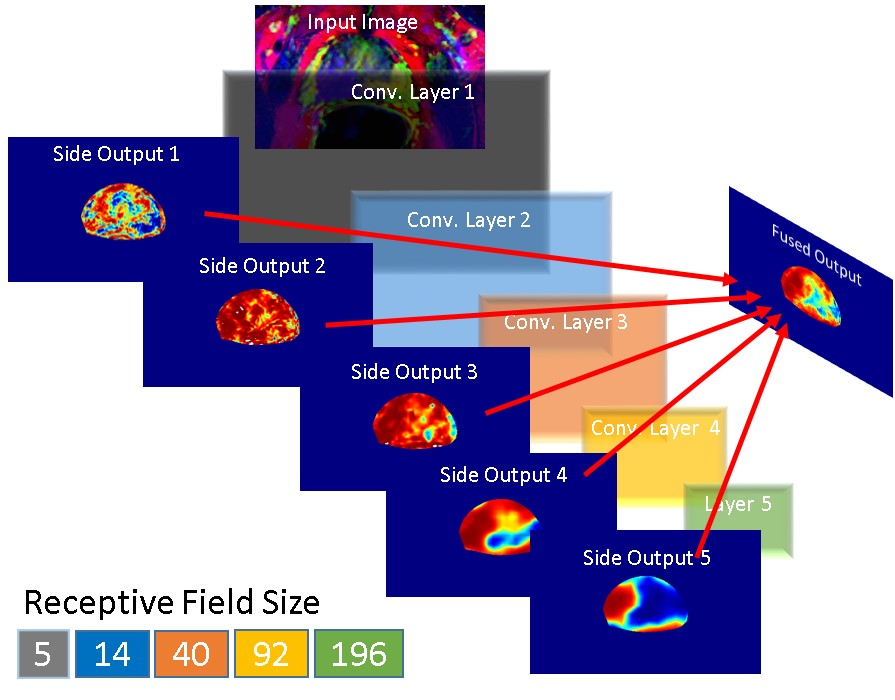
\includegraphics[height=8cm]{Figure4}
   \end{tabular}
   \end{center}
   \caption[Fig4]
   { \label{fig:Fig4} 
The adopted CNN architecture has 5 side outputs from 5 different convolutional layers each with a different receptive field. The five side outputs can be combined for a fused output.}
   \end{figure}
Inherent in its loss function is a balancing scheme that assigns weights for positive and negative loss outputs according to Equation~(\ref{eq:eq2}).
\begin{equation}
\label{eq:eq2}
\ell = - \frac{Y^{-}}{Y}\sum_{i\in Y^{+}} \log Pr(y_i=1|X) - \frac{Y^{+}}{Y} \sum_{i\in Y^{-}} \log Pr(y_i=0|X) \,,
\end{equation}
where $Y = \{y_i, i=1,...,|X|\}, y_i \in {0,1}$, $Y^{+}$ represent all pixels with positive labels, and $Y^{-}$ all with negative labels. The loss becomes zero for images with no positive labels such as those image slices with no marked tumors present. This feature reduces our training data set quite dramatically since a lesion on average maintains visibility on 3 slices and a patient's scan can have up to 30 slices. Therefore, we adjusted the balancing weight such that the total number of positive and negative labels in the entire training data-set are used for its computation.
\begin{equation}
\label{eq:eq3}
Y^{++} = \sum_{i}^{N}Y^{+}_{i} \,,and
\end{equation}
\begin{equation}
\label{eq:eq3}
Y^{--} = \sum_{i}^{N}Y^{-}_{i} \,,
\end{equation}
where $Y^{++}$ and $Y^{--}$ are the total number of positive and negative labels in the entire training-set, and $N$ is the total number of training examples. The resulting  coefficients are essentially global weights that are applied at every iteration during training. Hyper-parameters such as the learning-rate, gamma, momentum, and weight-decay were set to $1e-8$, $0.1$, $0.9$, and $0.0002$ respectively. During training, the weights were initialized using a pre-trained edge detection model, and Sigmoid-Cross-Entropy-Loss with stochastic gradient descent was used for optimization.

